\setAuthor{Siim Ainsaar}
\setRound{lahtine}
\setYear{2009}
\setNumber{G 10}
\setDifficulty{8}
\setTopic{Kinemaatika}

\prob{Müra}
Matkaja rõõmustab laagriplatsil, et elektrijaama müra tuuletu ilmaga nii vaikselt temani kostab. Hiljem, kui tuul tõuseb, on müra veel vaiksem. Puhub põhjatuul kiirusega $\beta c$, kus $c$ on heli kiirus paigalseisvas õhus; jaam jääb matkajast edelasse
(st tuule ja jaama suundade vaheline nurk on $\alpha = \ang{135}$).\\
\osa Kas helisagedus on sama mis tuuleta?\\
\osa Kui tuuleta on tajutav helivõimsus $P$ ja tuulega $xP$, siis kui suur on $x$?\\
Võite lugeda, et elektrijaam on punktikujuline. 

\emph{Soovitus:} uurige helifrondi levimist.

\hint
Ülesannet on mugavam vaadelda õhu taustsüsteemis, sest siis on helilainefrondid kiirusega $c$ kasvava raadiusega ja paigaloleva keskmega poolsfäärid. Helivõimsus jaotub ühtlaselt üle terve frondipinna, seega on tajutav võimsus pöördvõrdeline frondi pindalaga ehk frondi raadiuse ruuduga.

\solu
% Joonis
Õhu taustsüsteemis on helilainefrondid kiirusega $c$ kasvava raadiuse ja paigaloleva keskmega poolsfäärid. Helivõimsus jaotub ühtlaselt üle terve frondipinna, seega on tajutav võimsus pöördvõrdeline frondi pindalaga ehk pöördvõrdeline frondi raadiuse ruuduga. Lisaks on võimsus ka võrdeline frontide vastuvõtmise sagedusega ehk võrdeline helisagedusega, aga nagu peagi leiame, on sagedus konstant.

\begin{wrapfigure}{r}{0.5\linewidth}
	\vspace{-10pt}
	\begin{center}
		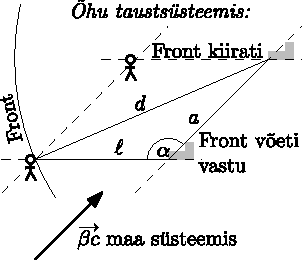
\includegraphics[width = 0.9\linewidth]{2009-lahg-10-lah}
	\end{center}
\end{wrapfigure}

Õhu taustsüsteemis liiguvad nii matkaja kui ka jaam vastu esialgsele tuule suunale kiirusega $\beta c$. Järelikult kui front oli vastuvõtmise hetkeks raadiusega $d = ct$, siis selle kiirgamise alguspunkt oli liikunud jaama suhtes allatuult kaugusele $a = (\beta c)t = \beta d$. Et see kaugus on kõigile frontidele ühesugune, on sama ka frontide teeloleku aeg ning aeg kahe frondi kiirgamise vahel võrdub ajaga nende vastuvõtmise vahel. Seega helisagedus ei muutu. Olgu jaama kaugus $\ell$. Rakendame tekkinud kolmnurgale koosinusteoreemi:
\[
d^{2}=a^{2}+\ell^{2}-2 a \ell \cos \alpha.
\]
Kuna $x = \left(\frac{\ell}{d}\right)^2$ ja $\cos \ang{135}=-\frac{\sqrt{2}}{2}$, saame $\sqrt x$ leidmiseks ruutvõrrandi, kusjuures $\ell$ taandub välja (karakteristlik pikkusmõõde puudub).
\[
\begin{array}{c}{\frac{\ell^{2}}{x}=\frac{\beta^{2} \ell^{2}}{x}+\ell^{2}+\frac{\sqrt{2} \beta \ell^{2}}{\sqrt{x}}} \\ {x+\sqrt{2} \beta \sqrt{x}+\beta^{2}-1=0} \\ {x=\left(\frac{-\sqrt{2} \beta \pm \sqrt{2 \beta^{2}-4 \beta^{2}+4}}{2}\right)^{2}=\frac{\left(-\beta \pm \sqrt{2-\beta^{2}}\right)^{2}}{2}=1 \mp \beta \sqrt{2-\beta^{2}}.}\end{array}
\]
Heli jääb vaiksemaks, mistõttu $x < 1$ ja peame valima miinusmärgiga lahend
\[
x=1-\beta \sqrt{2-\beta^{2}}.
\]
\probend